\documentclass[sigconf]{acmart}

\usepackage{booktabs} % For formal tables
\usepackage{amsmath}
\usepackage{tipa}
\usepackage{subcaption}
\usepackage{graphicx}
\usepackage{hyperref}
\usepackage{parskip}
\usepackage{minted}
\usepackage{xcolor}
% Copyright
\setcopyright{none}
%\setcopyright{acmcopyright}
%\setcopyright{acmlicensed}
%\setcopyright{rightsretained}
%\setcopyright{usgov}
%\setcopyright{usgovmixed}
%\setcopyright{cagov}
%\setcopyright{cagovmixed}


% DOI
\acmDOI{ }

% ISBN
\acmISBN{ }

%Conference
\acmConference[DTU]{DTU conference}{August 2017}{Kgs Lyngby, Denmark} 
\acmYear{1997}
\copyrightyear{2017}


\acmArticle{1}
\acmPrice{3.50}



\begin{document}
\title{Report 1 - Operating Systems}
%\titlenote{Produces the permission block, and copyright information}
\subtitle{Roar Nind Steffensen (s144107)}
%\subtitlenote{The full version of the author's guide is available as
%  \texttt{acmart.pdf} document}


%\author{Ben Trovato}
%\authornote{Dr.~Trovato insisted his name be first.}
%\orcid{1234-5678-9012}
%\affiliation{%
%  \institution{Institute for Clarity in Documentation}
%  \streetaddress{P.O. Box 1212}
%  \city{Dublin} 
%  \state{Ohio} 
%  \postcode{43017-6221}
%}
%\email{trovato@corporation.com}

% The default list of authors is too long for headers.
\renewcommand{\shortauthors}{B. Trovato et al.}

% These commands are optional
%\acmBooktitle{Transactions of the ACM Woodstock conference}
%\editor{Roar Nind Steffensen}

%\begin{abstract}
%This paper provides a sample of a \LaTeX\ document which conforms, somewhat loosely, to the formatting guidelines for ACM SIG Proceedings.\footnote{This is an abstract footnote}
%\end{abstract}

%
% The code below should be generated by the tool at
% http://dl.acm.org/ccs.cfm
% Please copy and paste the code instead of the example below. 
%
%\begin{CCSXML}
%<ccs2012>
% <concept>
%  <concept_id>10010520.10010553.10010562</concept_id>
%  <concept_desc>Computer systems organization~Embedded systems</concept_desc>
%  <concept_significance>500</concept_significance>
% </concept>
% <concept>
%  <concept_id>10010520.10010575.10010755</concept_id>
%  <concept_desc>Computer systems organization~Redundancy</concept_desc>
%  <concept_significance>300</concept_significance>
% </concept>
% <concept>
%  <concept_id>10010520.10010553.10010554</concept_id>
%  <concept_desc>Computer systems organization~Robotics</concept_desc>
%  <concept_significance>100</concept_significance>
% </concept>
% <concept>
%  <concept_id>10003033.10003083.10003095</concept_id>
%  <concept_desc>Networks~Network reliability</concept_desc>
%  <concept_significance>100</concept_significance>
% </concept>
%</ccs2012>  
%\end{CCSXML}

%\ccsdesc[500]{Computer systems organization~Embedded systems}
%\ccsdesc[300]{Computer systems organization~Redundancy}
%\ccsdesc{Computer systems organization~Robotics}
%\ccsdesc[100]{Networks~Network reliability}


\keywords{System Calls, C, Cache, Data Structures}



\maketitle

\section{Collection Week 3}

The requested program were to respond to the following single character input, as given in \cite{Ex3Instr}:

\begin{itemize}
    \item 'a': Add the current counter value to the collection, then increment the counter.
    \item 'b': Do nothing except increment the counter.
    \item 'c': Remove the most recently added element from the collection and increment the counter.
    \item Anything else: Stop processing commands, print the collection in the order they were added, and exit.
\end{itemize}

The choice of data structure, is in this case a linked list. The linked list is easy to expand dynamically at runtime, since only the new element requires memory to be allocated. The elements themselves are implemented using a struct containing pointers to the previous and next element, plus the value assigned. In this case the value of the counter as it is assigned.

At first, the collection is composed of one uninitialized element. Two pointers are used to keep track of the start and end of the list, named \texttt{head} and \texttt{current}. When a new element is added to the collection, memory is allocated for the next element while the element pointed to by \texttt{current} gets the current counter value, and pointers are corrected:

\begin{minted}
[
frame=lines,
framesep=2mm,
baselinestretch=1.2,
fontsize=\footnotesize,
linenos
]
{C}
if(c=='a')
{
  collection* next = (collection*)malloc(sizeof(collection));
  current->val = counter++;
  next->prev = current;
  current = current->next = next;
  continue;
}
\end{minted}

Likewise when an element is removed, the pointer \texttt{current} is decremented to the previous element (if possible), and the last element is freed in memory. Trivial actions like incrementing the counter are implemented but not discussed here. 

When the list is printed, a separate printing function called \texttt{printer} is invoked. The function is as seen in the following code snippet.

\begin{minted}
[
frame=lines,
framesep=2mm,
baselinestretch=1.2,
fontsize=\footnotesize,
linenos
]
{C}
void printer(collection* col)
{
  while(col->next)
    {
      write_int(col->val);
      col=col->next;
      if(col->next)
        write_char(',');
    }
  write_char('\n');
}
\end{minted}

The \texttt{printer} function checks if the last element is found, and if that is not the case, print out the value of the element, and increment the pointer. The last element in the list is uninitialized, and is therefore not printed, hence the \texttt{while(col->next)} condition.

The attached file \texttt{collectionweek3.c} contains the source code discussed.
\section{Cache Test Week 4}

When running the \texttt{cachetest.c} file, we get a list of times for different chache tests. From this, we will try to distinguish the cache line size, Li size, L2 size and L3 size.

If we analyze them in order, we first look for the cache line size. We suspect the read/write times to go up, as cache misses increase. When the stride length in the cachetest.c succeed our cache line size, more misses will occur, since the next procedure also misses subsequently. This should be clear when trying to allocate a large array, since the look-ups at cache misses will stand out. 

\begin{figure}[h]
    \centering
    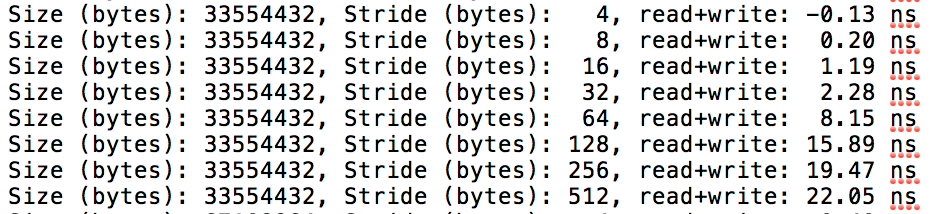
\includegraphics[width=\linewidth]{Week4/fig/CacheBlock.png}
    \caption{Times showing the cache line as the highest relative jump in time.}
    \label{fig:cacheblock}
\end{figure}

In fig \ref{fig:cacheblock} we see the biggest relative jump (\textbf{x}4) when going from a stride length of 32 bytes to 64 bytes. This suggests that our line size is either of theses two sizes, depending on how the line content is chosen when caching. 

Next step is to find the sizes of L1, L2 and L3 cache. If the complete array is stored in cache, the times should not go up no matter the stride length. When the data structure can no longer be contained in the different cache levels, the sizes of these cache levels should then be seen as a sudden spike in time (most significant when stride succeeds the cache line size). The stride lengths are not shown in fig \ref{fig:misses}, but the ordering is not altered compared to fig \ref{fig:cacheblock}.

\begin{figure}[ht]
\centering
    \begin{subfigure}{0.4\textwidth}
    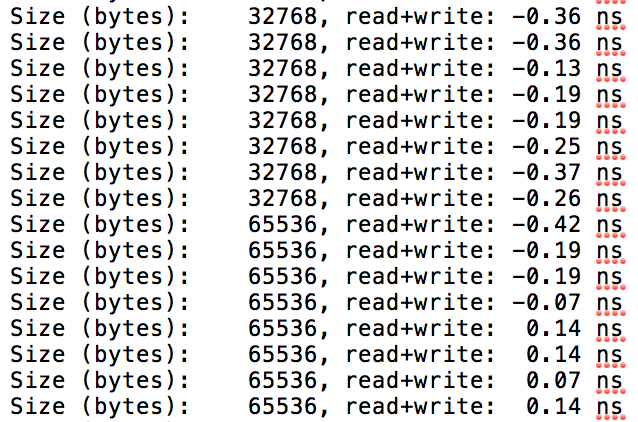
\includegraphics[width=\linewidth]{Week4/fig/L1Miss.png} 
    \caption{ }
    \label{fig:L1}
    \end{subfigure} 
    
    \begin{subfigure}{0.4\textwidth}
    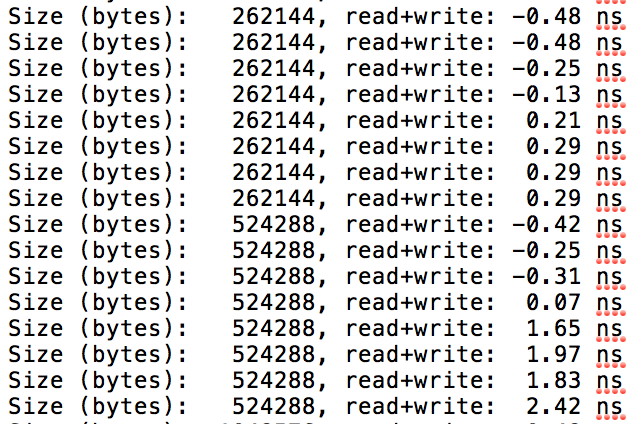
\includegraphics[width=\linewidth]{Week4/fig/L2Miss.png}
    \caption{ }
    \label{fig:L2}
    \end{subfigure}
    
    \begin{subfigure}{0.4\textwidth}
    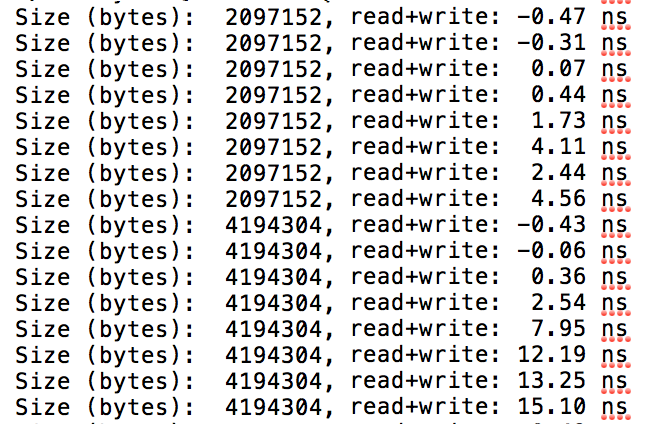
\includegraphics[width=\linewidth]{Week4/fig/L3Miss.png}
    \caption{ }
    \label{fig:L3}
    \end{subfigure}
    
    \caption{Cache misses showing: a) L1 limit, b) L2 limit and c) L3 limit.}
    \label{fig:misses}
\end{figure}

As seen in fig \ref{fig:L1}, the first jump in time is from 32kB to 64kB, suggesting that this system has a L1 cache size of around 32kB. Using the same reasoning fig \ref{fig:L2} and \ref{fig:L3} suggest that the L2 cache size is around 258kB and L3 cache size is around 2MB or 3MB. 

Looking up the computer specifications, we see that indeed the cache line size is 64 bytes, L1 has size 32kB (each of dcache and ichache), L2 has size 258kB and L3 has size 3MB. 

To alter the \texttt{cachetest.c} file for better read/write speeds, we need to make sure, that subsequent operations optimize for reusing cached memory. In the first do-while loop, the two for-loops control how the memory is accessed in the array \texttt{x}. The innermost loop increments the index by the stride length. This means, that every look-up is at a new position. If the two for loops change order, the index is constant for every iteration of the innermost loop. This will minimize cache misses, since two subsequently look-ups of the same memory, is \textit{almost} guaranteed to be cached. Running the program again, we see that all the times are now below 0.4 ns. 

This means, in order to optimize future programs for cache, we need to take the sizes of L1 to L3 cache into consideration when creating data structures. If an array is used, which can be fully stored e.g. in the 32kB L1 dcache, together with the various local variables, memory access would be optimal. If larger data structures are needed, the size of the cache line (in this case 64 bytes) is important, since the subsequent memory accesses' would be contained in the cache line, if the information is contained from the loaded memory block in the cache line. In general cache hits would also be likely when reusing variables, instead of accessing new memory addresses each time (or rather, the the address modulus the number of cache lines $32\text{kB}/64\text{B} = 500$ for L1 if directly mapped). Most operating systems don't use directly mapped cache, but instead a form of set-associative caching. This means, that conflicts in cached memory is less, and the general strategy is; grouping variables, and accessing data with short intervals, optimizing for space and time locality. 

The attached file \texttt{cachetest.c} containes the source code discussed.
\section{Colletion Week 4}

Instead of using \texttt{getchar()} and \texttt{printf()}, input and output should now be handled using the provided linux system calls from the \texttt{io.c} and \texttt{io.h} files. Since the function \texttt{syscall\_read()} can be used directly to read characters, much like \texttt{scanf()}, the substitution cause little change in the code, and the focus in this report will instead be directed towards output.


The original program from week 3 iterates over the linked list, and prints out the elements sequentially. This means, that we only have to worry about printing an integer (and a comma). 

Since the integer can span over several characters, the amount of digits must first be evaluated. This is done using integer division by 10 as long as the number is larger than 9. Counting the amount of divisions gives us the amount digits the integer contains.\footnote{Since the divisions stop at the last digit, the we add 1 to the count to get the correct amount.} With the amount of digits, we can initialize an array of characters. We then go through the original integer again (using modulus and integer division by 10) adding the characters to the array in reverse order. This leaves us with an array containing the number as the corresponding characters. \texttt{syscall\_write()} can then be used to print the number. This can be seen in the code in fig \ref{fig:intprint}.

\begin{figure}[ht]
\centering
\begin{minted}
[
frame=lines,
framesep=2mm,
baselinestretch=1.2,
fontsize=\footnotesize,
linenos
]
{C}
int write_int(int value) {
  int tmp = value;
  int size = 1;
  
  while(tmp > 9){
    tmp /= 10;
    size++;
  }

  char chrs[size];
  int i;
  for(i =size-1; i >= 0; i--) {
    chrs[i] = (char)((value % 10) + '0');
    value /= 10;
  }

  syscall_write(chrs, size);
}

\end{minted}
\caption{Integer printing function}
\label{fig:intprint}
\end{figure}

After printing a number, it is checked if the end of the list is reached; if not, a comma is printed using the helper function \texttt{write\_char()}. 

With these alterations to the program, the only external functions are \texttt{malloc()} and \texttt{free()} from \texttt{stdlib.h}, as was the goal of the assignment.

If we check the \texttt{sizeof} of the struct \texttt{collection} we see that it is 24 bytes, meaning that a link can be fully loaded into cache within a single cache line. As it is not known how vigorous this algorithm will be used, and if the list itself will be larger than what is possible to store in cache, it is good that each element themselves can be read with at most one cache miss.


The attached files \texttt{collectionweek4}, \texttt{io.c} and \texttt{io.h} contain the source code discussed.
\section{Compilation Flow}

During the compilation process of a c program, several steps are performed. These steps can be divided up into 

\begin{itemize}
    \item Preprocessor
    \item Compiler
    \item Assembler
    \item Linker
\end{itemize}

respectively. 

The \texttt{Preprocesssor} takes the \texttt{.c} file, and follow the instructions beginning with a $\#$. This procedure involves including library/other files, substitution of macros, and based on conditions omit code and e.g. strip comments. The preprocessing step prepares the file and syntax for the "Compile" step, in form of a translation unit. 

The \texttt{Compiler} compiles the translation unit into assembly instructions specific for the environment/processor architecture. If specified, some optimizations may occur. Optimizations may involve how/when data is accessed and/or the size of the compiled code.

The \texttt{Assembler} converts the assembly instructions directly into machine code in an object file. The object file therefore contains binary instructions also specific for the processor architecture. 

The \texttt{Linker} makes sure, that all objects or pieces of code e.g. from libraries are collected in the final executable file/program.

\bibliographystyle{ACM-Reference-Format}
\bibliography{sample-bibliography} 

\end{document}
